%%%%%%%%%%%%%%%%%%%%%%%%%%%%%%%%%%%%%%%%%
% baposter Landscape Poster
% LaTeX Template
% Version 1.0 (11/06/13)
%
% baposter Class Created by:
% Brian Amberg (baposter@brian-amberg.de)
%
% This template has been downloaded from:
% http://www.LaTeXTemplates.com
%
% License:
% CC BY-NC-SA 3.0 (http://creativecommons.org/licenses/by-nc-sa/3.0/)
%
%%%%%%%%%%%%%%%%%%%%%%%%%%%%%%%%%%%%%%%%%

%----------------------------------------------------------------------------------------
%	PACKAGES AND OTHER DOCUMENT CONFIGURATIONS
%----------------------------------------------------------------------------------------

\documentclass[landscape,a0paper,fontscale=0.285]{baposter} % Adjust the font scale/size here

\usepackage{graphicx} % Required for including images
\graphicspath{{figures/}} % Directory in which figures are stored

\usepackage{amsmath} % For typesetting math
\usepackage{amssymb} % Adds new symbols to be used in math mode

\usepackage{booktabs} % Top and bottom rules for tables
\usepackage{enumitem} % Used to reduce itemize/enumerate spacing
\usepackage{palatino} % Use the Palatino font
\usepackage[font=small,labelfont=bf]{caption} % Required for specifying captions to tables and figures

\usepackage{multicol} % Required for multiple columns
\setlength{\columnsep}{1.5em} % Slightly increase the space between columns
\setlength{\columnseprule}{0mm} % No horizontal rule between columns

\usepackage{tikz} % Required for flow chart
\usetikzlibrary{shapes,arrows} % Tikz libraries required for the flow chart in the template

\newcommand{\compresslist}{ % Define a command to reduce spacing within itemize/enumerate environments, this is used right after \begin{itemize} or \begin{enumerate}
\setlength{\itemsep}{1pt}
\setlength{\parskip}{0pt}
\setlength{\parsep}{0pt}
}

\definecolor{lightblue}{rgb}{0.145,0.6666,1} % Defines the color used for content box headers

\newcommand\e{\emph}
\newcommand\tb{\textbf}
\newcommand\un{\underline}
\newcommand\txt{\texttt}

\usepackage{float}
\usepackage{hyperref}

\begin{document}

\begin{poster}
{
headerborder=closed, % Adds a border around the header of content boxes
colspacing=1em, % Column spacing
bgColorOne=white, % Background color for the gradient on the left side of the poster
bgColorTwo=white, % Background color for the gradient on the right side of the poster
borderColor=lightblue, % Border color
headerColorOne=black, % Background color for the header in the content boxes (left side)
headerColorTwo=lightblue, % Background color for the header in the content boxes (right side)
headerFontColor=white, % Text color for the header text in the content boxes
boxColorOne=white, % Background color of the content boxes
textborder=roundedleft, % Format of the border around content boxes, can be: none, bars, coils, triangles, rectangle, rounded, roundedsmall, roundedright or faded
eyecatcher=true, % Set to false for ignoring the left logo in the title and move the title left
headerheight=0.1\textheight, % Height of the header
headershape=roundedright, % Specify the rounded corner in the content box headers, can be: rectangle, small-rounded, roundedright, roundedleft or rounded
headerfont=\Large\bf\textsc, % Large, bold and sans serif font in the headers of content boxes
%textfont={\setlength{\parindent}{1.5em}}, % Uncomment for paragraph indentation
linewidth=2pt % Width of the border lines around content boxes
}
%----------------------------------------------------------------------------------------
%	TITLE SECTION 
%----------------------------------------------------------------------------------------
%
{
\includegraphics[height=4em]{logo.png}} % First university/lab logo on the left
{\bf\textsc{Will God's Grace Guide My Vote?}\smallskip} % Poster title
{\textsc{{\LARGE\tb{Jennifer Lin and Steven M. Graham} } \smallskip\\ New College of Florida, Department of Psychology}} % Author names and institution
{
\includegraphics[height=4em]{logo}} % Second university/lab logo on the right

%----------------------------------------------------------------------------------------
%	OBJECTIVES
%----------------------------------------------------------------------------------------

\headerbox{Guiding Questions}{name=objectives,column=0,row=0}{

Elections often happen in public places, including many Houses of Worship. This project aims to understand the relationship between primes of religion and its influence on political attitudes. 

\begin{enumerate}
	\item Do subliminal religious primes influence political decision-making?
	\item If yes, in which direction on the left-right scale?
\end{enumerate}

\vspace{0.3em} % When there are two boxes, some whitespace may need to be added if the one on the right has more content
}

%----------------------------------------------------------------------------------------
%	INTRODUCTION
%----------------------------------------------------------------------------------------

\headerbox{Hypotheses}{name=introduction,column=1,row=0,bottomaligned=objectives}{

The hypotheses for the study were made from information in past research regarding the voting patterns of religious individuals. Since a growing number of religious people lean Republican, the hypotheses reflect this trend.

\begin{enumerate}\compresslist
	\item Religious primes influence political decisions
	\item People think more conservatively in the religious mindset
\end{enumerate}
}

%----------------------------------------------------------------------------------------
%	RESULTS 1
%----------------------------------------------------------------------------------------

\headerbox{Results}{name=results,column=2,span=2,row=0}{

\begin{multicols}{2}
\vspace{1em}
%\begin{center}
%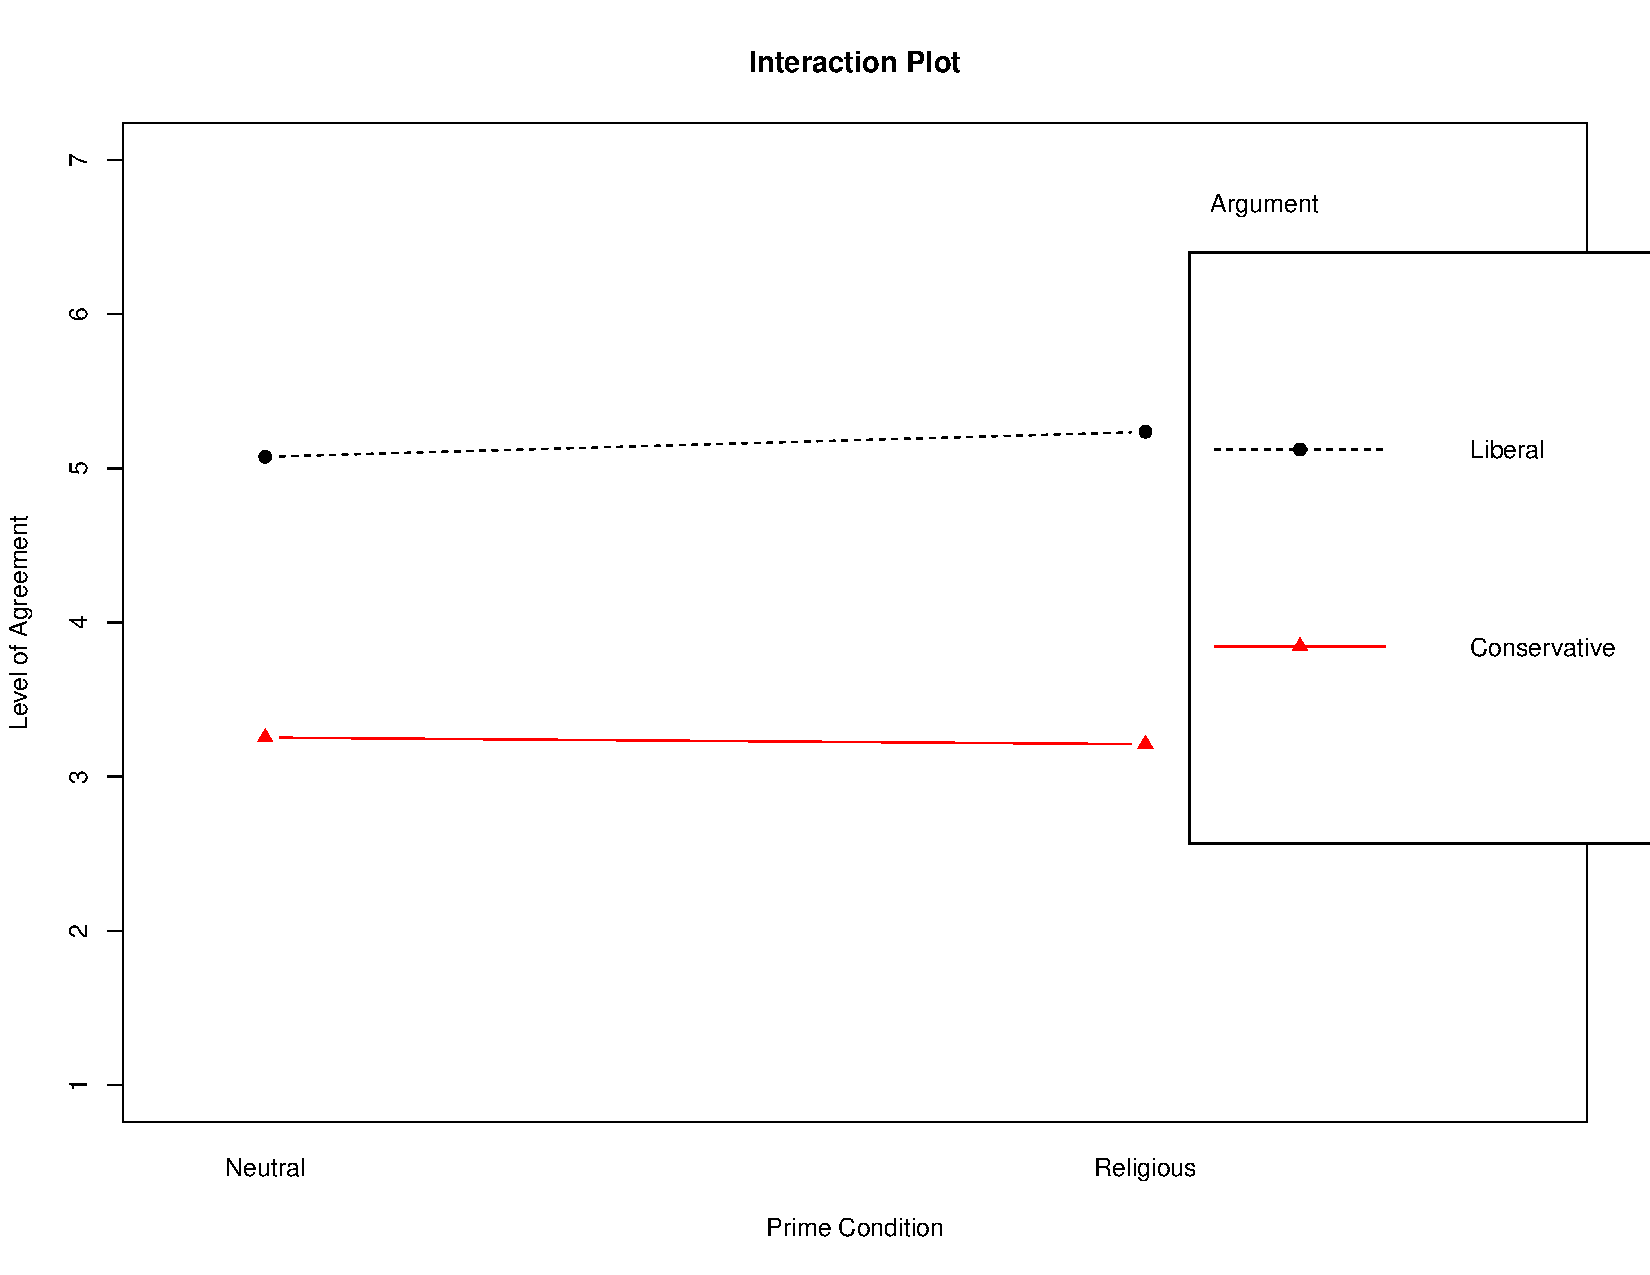
\includegraphics[width=0.8\linewidth]{InteractionPlot}
%\captionof{figure}{Figure caption}
%\end{center}

\tb{Description of Participants}

\begin{itemize}\compresslist
	\item The majority (n = 172) identified as non-religious
	\item Most identified with the Democrat party (n = 137)
	\item 217 participants identified as 40 or younger
\end{itemize}

\tb{Method of Analysis}

\begin{itemize} \compresslist
	\item 2 (Prime Condition: Religious or Neutral) $\times$ 2 (Issue Condition: Liberal or Conservative) ANOVA - Between-Subjects design
	\item $\alpha = .05$
\end{itemize}
\end{multicols}

%------------------------------------------------

\begin{multicols}{2}
\vspace{1em}
\begin{table}[H]
	\centering
	\caption{Results for 2 $\times$ 2 ANOVA}
	\small
	\begin{tabular}{lccccc}
		\hline
		\tb{Variables}&\tb{df}&\tb{SS}&\tb{MS}&\tb{F}&\tb{p-value}\\
		\hline
		Prime&1&0.00&0.00&0.00&0.984\\
		Argument&1&280.00&280.03&56.22&0.001***\\
		Interaction&1&0.8&0.79&0.159&0.690\\
		Residuals&299&1489.00&4.98&&\\
		\hline
	\end{tabular}\\
	Note: * p$<$0.05; ** p$<$0.01; *** p$<$0.001
\end{table}


\begin{itemize} \compresslist
	\item No Interaction for Religious Prime and Argument (\e{F}(1,299) = 0.159, \e{p} = .69, $\eta^{2}$ = .00)
	\item No main effect of Religious Prime (\e{F}(1,299) = 0.00, \e{p} = .98, $\eta^{2}$ = .00)
	\item Main effect of Argument (\e{F}(1,299) = 56.22, \e{p} = .001, $\eta^{2}$ = .16)
\end{itemize}

\begin{center}
\begin{figure}[H] \centering
	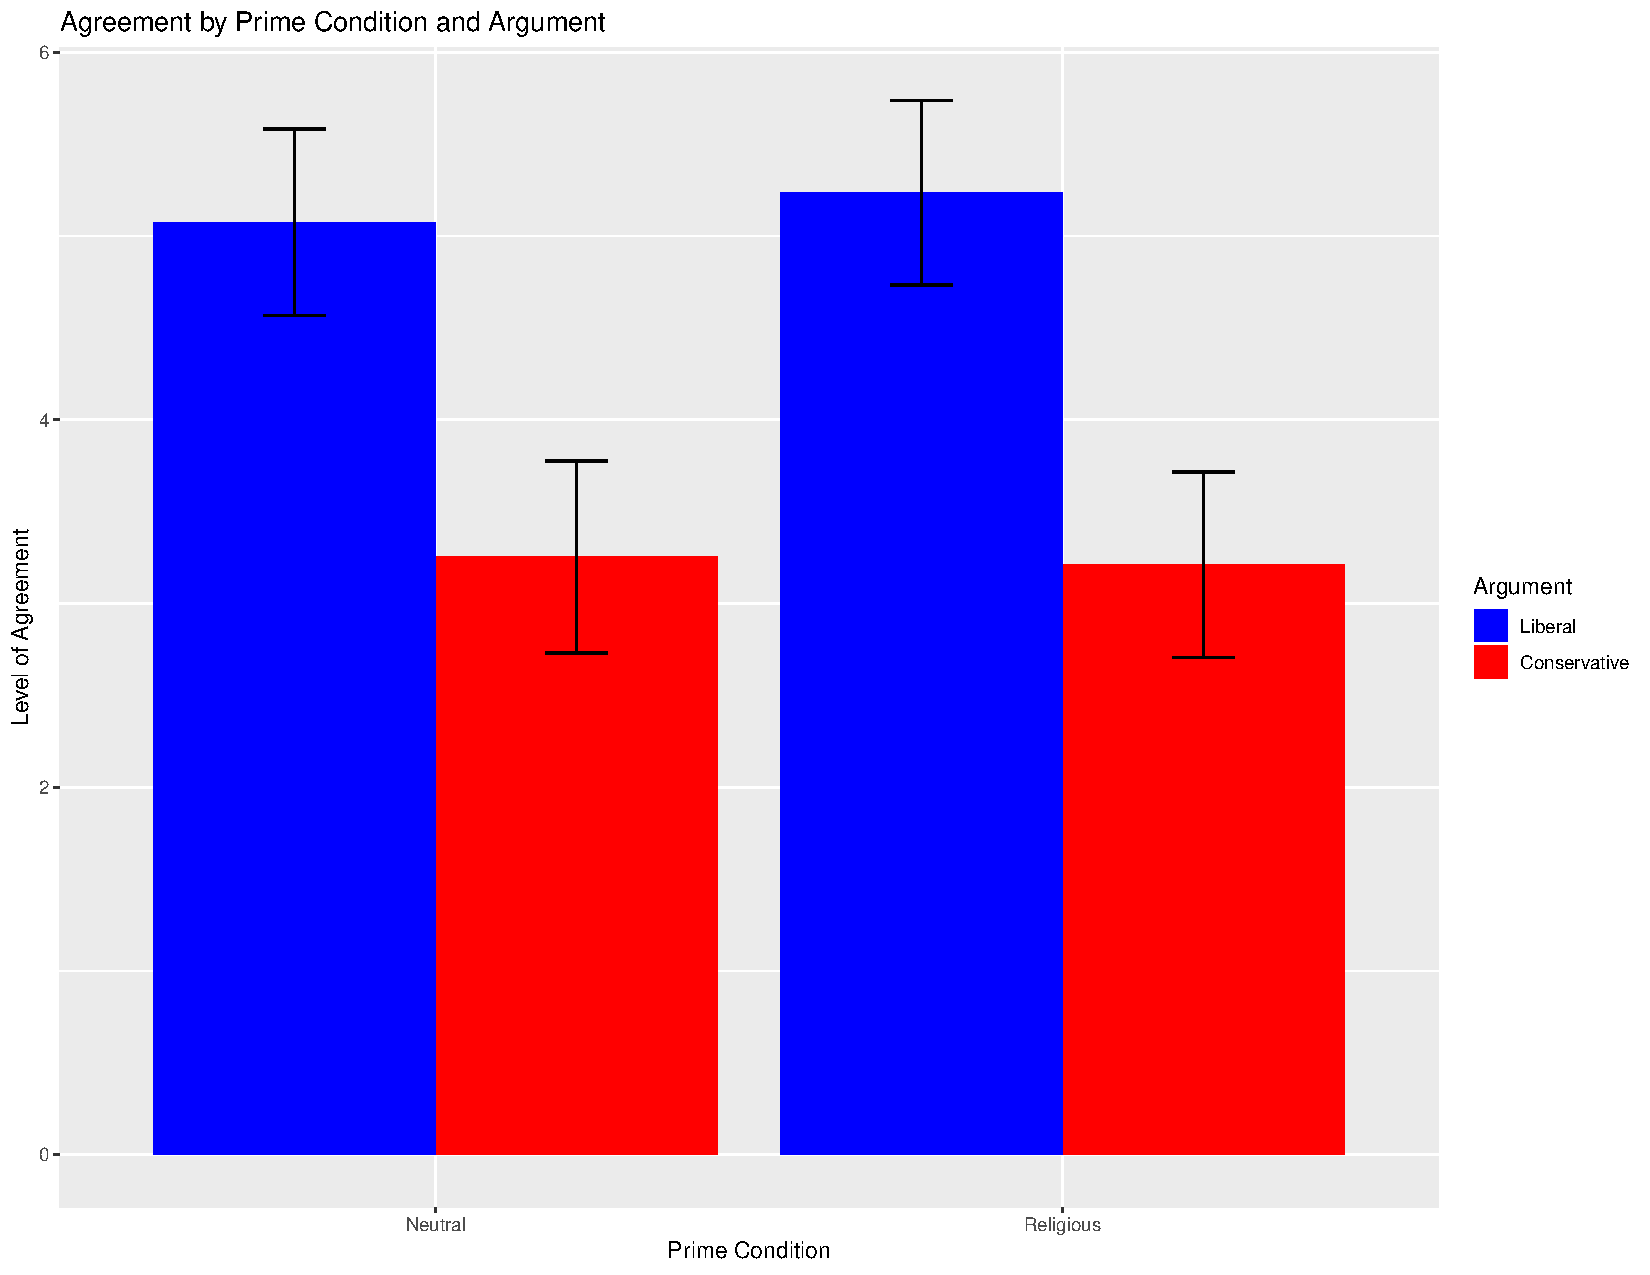
\includegraphics[width=0.8\linewidth]{barplot} 
	\captionsetup{justification=centering}
	\captionof{figure}{Responses to Argument by Prime Condition}
\end{figure}

\end{center}

\end{multicols}
}

%----------------------------------------------------------------------------------------
%	REFERENCES
%----------------------------------------------------------------------------------------

\headerbox{Select Bibliography}{name=references,column=0,above=bottom}{

\renewcommand{\section}[2]{\vskip 0.05em} % Get rid of the default "References" section title
\nocite{*} % Insert publications even if they are not cited in the poster
\footnotesize{ % Reduce the font size in this block
\bibliographystyle{unsrt}
\bibliography{poster} % Use sample.bib as the bibliography file
}}

%----------------------------------------------------------------------------------------
%	FUTURE RESEARCH
%----------------------------------------------------------------------------------------

\headerbox{Future Research}{name=futureresearch,column=1,span=2,aligned=references,above=bottom}{ % This block is as tall as the references block

\begin{multicols}{2}
\begin{itemize} \compresslist
	\item Analyze voter files and precinct returns to link people who voted in precincts with the percentage of people who vote on down ballot candidates. 
	\item In future experiments, use of a less polarizing subject as manipulation so that people would not enter the study with preconceived notions about the topic, which were largely reflected in their qualitative responses
\end{itemize}
\end{multicols}
}

%----------------------------------------------------------------------------------------
%	CONTACT INFORMATION
%----------------------------------------------------------------------------------------

\headerbox{Contact Information}{name=contact,column=3,aligned=references,above=bottom}{ % This block is as tall as the references block

\begin{description}\compresslist
\item[Web] www.ncf.edu
\item[Email] \href{mailto:jennifer.lin16@ncf.edu}{jennifer.lin16@ncf.edu} $\mid$ \href{mailto:sgraham@ncf.edu}{sgraham@ncf.edu}
\item[Phone] +1 (941) 487 5000
\item[Address] 5800 Bay Shore Road Sarasota, FL 34243
\end{description}
}

%----------------------------------------------------------------------------------------
%	CONCLUSION
%----------------------------------------------------------------------------------------

\headerbox{Conclusion}{name=conclusion,column=2,span=2,row=0,below=results,above=references}{

\begin{multicols}{2}

\tb{Findings from the Study}
\begin{itemize} \compresslist
	\item Religious primes did not influence vote choice -- No matter what priming condition participants were in, they were equally likely to voice support or reject the argument
	\item Main effect present on Argument variable - Participants seemed to carry preconceptions on the topic based on ideology
	\item Agreement on the issue did not depend on the prime or argument condition
\end{itemize} 

\tb{Limitations of the Study}

\begin{itemize}\compresslist
	\item \tb{Amazon Mechanical Turk:} The participants were relatively more liberal and secular, leading to a natural tendency to favor the liberal side of the argument.
	\item \tb{The Topic:} People have relatively robust stances on abortion. Future iterations can analyze how people react to topics that are less debated, with religious primes added to the experiment. 
\end{itemize}



\end{multicols}
}

%----------------------------------------------------------------------------------------
%	MATERIALS AND METHODS
%----------------------------------------------------------------------------------------

\headerbox{Previous Research}{name=method,column=0,below=objectives,bottomaligned=conclusion}{ % This block's bottom aligns with the bottom of the conclusion block

\begin{itemize}
	\item Voting in churches can serve as reminders to people's faiths and subliminally prime their political stances \cite{berger_contextual_2008}.
	\item Americans are religious individuals, with 85\% of people identifying with a major denomination of worship \cite{putnam_american_2010}.
	\item As such, religion becomes a part of identity that can influence political decisions. Since religions teach people about living moral lives, this world view can be applied to understanding how politics ought to be.
	\item Often, politicians incorporate overt or subtle religious messages in their campaigns to attract people of faith to their cause.
	\item Likewise, preachers often instruct their followers to ``go with the Word" before elections \cite{putnam_american_2010}, which can influence the votes of the parishioners. 
	\item High costs of voting leads voters to be susceptible to primes and heuristics \cite{berger_contextual_2008}. 
\end{itemize}

  
}

%----------------------------------------------------------------------------------------
%	RESULTS 2
%----------------------------------------------------------------------------------------

\headerbox{Materials \& Methods}{name=results2,column=1,below=objectives,bottomaligned=conclusion}{ % This block's bottom aligns with the bottom of the conclusion block

\tb{Participants and Recruitment: }
\begin{itemize} \compresslist
	\item 304 of 356 original respondents incorporated in analysis (133 identify as female)
	\item Recruited via Amazon Mechanical Turk
	\item Participants were paid \$1 for their participation
\end{itemize}

\tb{Experiment Tasks:}

\begin{itemize} \compresslist
	\item \tb{Sentence Reorganization} -- Participants saw 5 word chunks (of religious or neutral content) and had to rearrange them to make logical sentences.
	\item \tb{Statement and Agreement on Controversial Issue} -- Participants read vignettes supporting or countering abortion and were asked to rate the quality of the argument along with the extent they agreed
	\item \tb{Religiosity Measure} -- Survey on religious identity
	\item \tb{Demographic Questions} -- Questions include race, gender, and political affiliation 
	\item \tb{Manipulation Check}
\end{itemize}
}

%----------------------------------------------------------------------------------------

\end{poster}

\end{document}